% !TEX encoding = UTF-8 Unicode

\documentclass[a4paper]{article}

\usepackage{xcolor}
\usepackage{url}
\usepackage[T2A]{fontenc} % enable Cyrillic fonts
\usepackage[utf8]{inputenc} % make weird characters work
\usepackage[margin=1in]{geometry}
\usepackage[serbianc]{babel}
\usepackage{CJKutf8}
\usepackage{graphicx}
\usepackage{fancyhdr}
\usepackage{listings}
\usepackage{csvsimple}
\usepackage{pgfplotstable}
\usepackage{longtable}
\usepackage{float}
\usepackage{amssymb}
\usepackage{amsthm}
\usepackage{mathtools}
\newtheorem{example}{Пример}
\newtheorem{theorem}{Теорема}
\newtheorem{definition}{Дефиниција}
\DeclareMathOperator{\mex}{mex}
% set the default code style

\definecolor{ghostwhite}{rgb}{0.98, 0.98, 0.98}
\definecolor{mediumviolet-red}{rgb}{0.78, 0.08, 0.52}
\definecolor{hooker\'sgreen}{rgb}{0.0, 0.44, 0.0}
\lstset{
	language=C++,
	breaklines=true,
	backgroundcolor=\color{ghostwhite},
	frame=tb, % draw a frame at the top and bottom of the code block
	tabsize=2, % tab space width
	showstringspaces=false, % don't mark spaces in strings
	numbers=left, % display line numbers on the left
	numberstyle=\color{gray},
	rulecolor=\color{black},
	keywordstyle=\color{mediumviolet-red}, % keyword color
	commentstyle=\color{hooker\'sgreen} %comment color
}
%\usepackage[english,serbianc]{babel} %ukljuciti babel sa ovim opcijama, umesto gornjim, ukoliko se koristi cirilica

\usepackage[unicode]{hyperref}
\hypersetup{colorlinks,citecolor=green,filecolor=green,linkcolor=blue,urlcolor=blue}

\pagestyle{fancy}
\fancyhf{}
\renewcommand{\headrulewidth}{0pt}
\fancyfoot[R]{\thepage}

\graphicspath{{./src/statistics/picture/}}

\begin{document}
\begin{titlepage}
    \begin{center}
        \vspace{0.5cm}
        
        \Large{
	        Универзитет у Београду\\
	        Математички факултет\\
        }
    
        \vspace{0.5cm}
        \Large{Мастер рад}    
        
        \vspace{2.0cm}
        
        \Huge
        \rule[0.5cm]{\textwidth}{0.5pt}
        \textbf{Игра ним}
        \rule{\textwidth}{0.5pt}
        \vspace{0.5cm}
        
        \vspace{2.0cm}
        
        \begin{minipage}[t]{0.47\textwidth}
        	\textnormal{\large{\bf Аутор:\\}}
        	{\large Марија Мијаиловић}
        \end{minipage}\hfill\begin{minipage}[t]{0.47\textwidth}\raggedleft
        	\textnormal{\large{\bf Ментор:\\}}
        	{\large Др Миодраг Живковић}
        \end{minipage}
        
        \vfill
        
        {\Large Катедра за рачунарство и информатику}
        
        \vspace{0.8cm}
        
        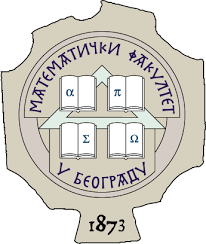
\includegraphics[width=0.3\textwidth]{matf_logo.png}
        
        \large{Београд, мај 2020}
        
    \end{center}
\end{titlepage}
\newpage
\pagenumbering{roman}
\tableofcontents

\newpage
\pagenumbering{arabic}
\section{Увод}
\label{sec:uvod}

\section{Ним}
\label{sec:nim}

Традиционална ним игра се игра у два играча са било којим предметима( новчићи, жетони, шибице, карте, ...), груписаних у гомиле. Број предмета и гомила је произвољан, тачније одређују их сами играчи. Играч који је на потезу може узети произвољан број жетона са једне гомиле, при чему мора узети бар један жетон и не сме узимати жетоне са више гомила. Играчи наизменично играју потезе. Како постоје нормалан и мизерни ним тип игре, постоје различити начини на које играч може да победи. У нормалном ниму побеђује играч који узме последњи жетон, док у мизерном губи играч који узме последњи жетон.

\begin{example}
На почетку партије на столу су три гомиле, са три, четири и пет жетона респективно. Партију играју два играча \textit{А} и \textit{Б}, \textit{А} игра први. 
\end{example}

Могући ток игре нормалног нима је приказан на слици \ref{fig:nimPrimer}.

\begin{figure}[H]
	\caption{Ток игре ним}
	\label{fig:nimPrimer}
	\begin{center}
		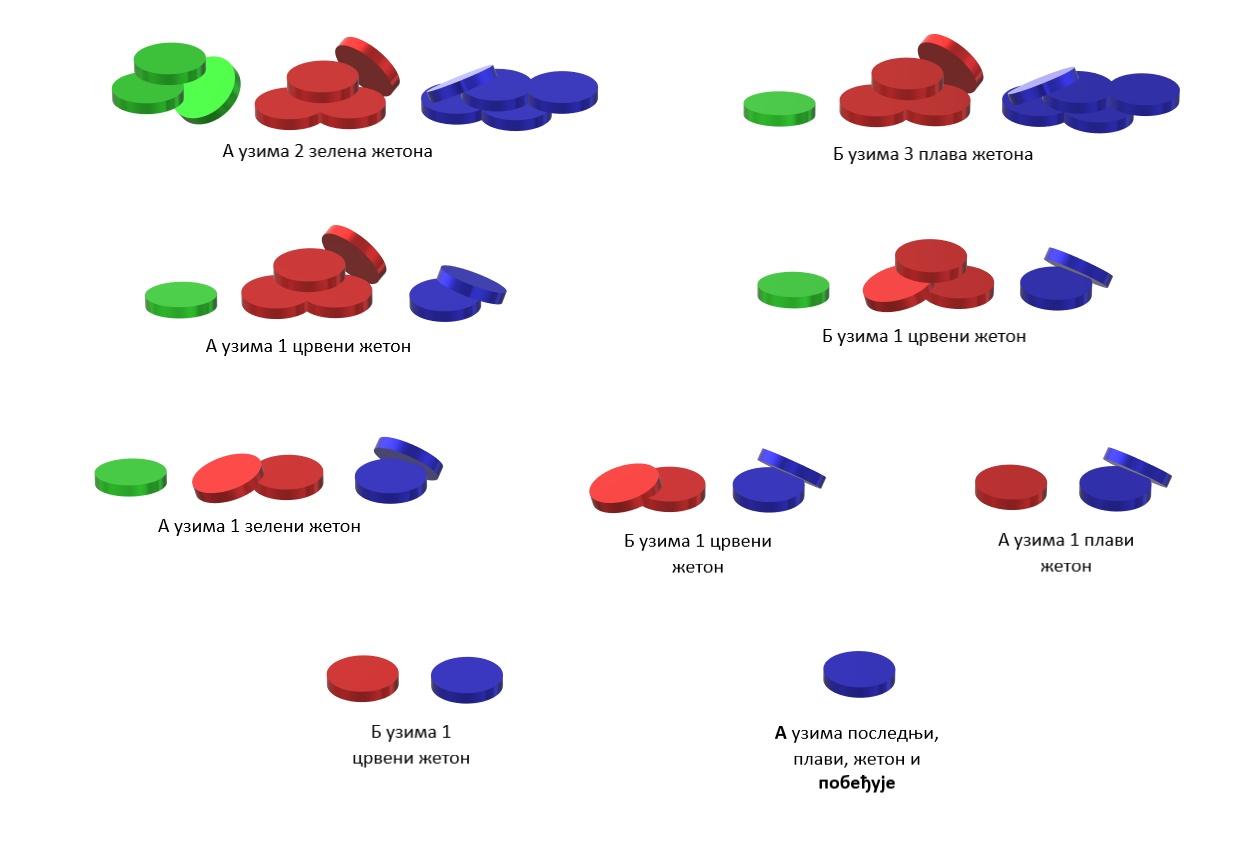
\includegraphics[width=\textwidth]{NimPrimer.png}
	\end{center}
\end{figure}

У општем случају, уколико се на столу налазе две гомиле, у зависности од броја жетона могући су следећи исходи нормалног нима:

\begin{itemize}
	\item Дате су две гомиле са по једним жетоном. Први играч мора да узме бар један жетон, чиме оставља другом играчу да узме последњи жетон и победи. У овој ситуацији очигледно је да \textbf{први играч загарантовано губи}.
	
	\item Дате су две гомиле, на првој један жетон, на другој два жетона. \textbf{Први играч има стратегију за победу}, уколико узме један жетон са гомиле где су нам два жетона (на слици \ref{fig:nimPrimer} узима 1 плави жетон), оставља следећем играчу две гомиле са по жетоном, а из претходног примера видели смо да је то стање у коме играч који је на потезу губи.
	
	\item Дате су две гомиле са по два жетона. Прва могућност јесте да први играч узме све са једне гомиле, чиме други играч истим тим потезом, узимајући све жетоне са друге гомиле, побеђује. Друга могућност је да први играч узме један жетон, тако да је следеће стање игре заправо стање из претходног примера, у коме играч који је на потезу побеђује. У овој ситуацији загарантовано је да \textbf{први играч губи}.
\end{itemize}

Сада би требало да је јасно да у овој игри нема среће, већ да се најбољи потез може направити само ако се предвиди редослед потеза који ће уследити. Очигледно је да постоји неки образац који ће нам за конкретан број жетона и гомила рећи начин игре који ће играча довести до победе. Амерички математичар Чарлс Бутон (енг. {~\em Charles Bouton}) је извршио комплетну математичку анализу игре и 1902 године је пронашао трик. \cite{10.2307/1967631}

\section{Витхофова игра}
\label{sec:vithofova_igra}

Постоје многе варијанте нима, које се од оригиналне верзије углавном разликују по томе што садрже бар једно додатно правило за игру. Једна таква верзија је Витхофова игра (енг.{~\em Wythoff's game})\cite{10.2307/2321643}.

Витхофова игра је математичка стратешка игра за два играча. На столу се налазе две гомиле жетона; Играчи наизменично узимају жетоне са једне или обе гомиле. Приликом узимања жетона са обе гомилe, рецимо $ k (> 0) $ са једне и $ l (> 0) $ са друге, мора да буде испуњен услов $ |k - l| < a $, где је $ a $ задати позитиван број. Игра се завршава када број жетона на талону буде нула, а онај играч који је уклонио последњи жетон или жетоне је победник. Сваки играч када је на потезу мора да уклони бар један жетон.

У класичној Витхоф игри $ a $ je $ 1 $, што значи да ако играч узима жетоне са обе гомиле, број узетих жетона мора бити једнак.

Игра се еквивалентно може описати и као игра са краљицом на шаховској табли: Имамо једну шаховску краљицу постављну било где на табли, сваки играч може да помера краљицу произвољан број корака у правцу југа, запада, или југозапада. Победник је играч који први помери краљицу у доњи леви угао табле.\cite{cut-the-knot, singingbanana-youtube}

Забележено је да се ова игра играла у Кини  под именом "\begin{CJK}{UTF8}{gbsn}捡石子\end{CJK} jiǎn shízǐ"(енг.{~\em picking stones}). \cite{Yaglom}

Холандски математичар В. А. Витхоф ({\em W. A. Wythoff}) је 1907. године објавио математичку анализу ове игре. \cite{wythoff1907modification}

\section{Оптимална стратегија}
\label{sec:optimalna_strategija}

Било која позиција се може представити паром бројева $ (a, b) $, где је $ a \le  b $, док  $ a $ и $ b $ представљају бројеве жетона на две гомиле или координате позиције краљице (при чему су координате доњег левог угла (0, 0)). Све могуће позиције могу се разврстати у две категорије, П-позиције и Н-позиције. 
\begin{definition}
	На П-позицји, играч који је на потезу губи ако противник игра како треба, другим речима наредни играч може да победи шта год одиграо противник. На Н-позицији, играч који је на потезу побеђује ако игра како треба.
\end{definition}

Класификација позиција на П и Н се дефинише рекурзивно на следећи начин:
\begin{enumerate}
	\item $ (0, 0) $ је П-позиција јер играч који је на потезу не може да одигра ниједан валидан потез, па је његов противник победник.
	\item Било која позиција са које је П-позиција достижна у једном потезу је Н-позиција. 
	\item Ако сваки потез води ка некој Н-позицији, онда је то П-позиција.
\end{enumerate}

Да би се Витхофова игра ирала на најбољи могући начин, потребно је знати две ствари:
\begin{itemize}
	\item Препознати природу тренутне позиције, да ли је П или Н
	\item Уколико је тренутна позиција Н, треба израчунати следећи потез тако да се противник нађе у П позицији.
\end{itemize}

Разлог битности лежи у чињеници да уколико је тренутна позиција Н, знамо да постоји потез који нас води на П-позицију, а тај потез можемо израчунати и победити. Са друге стране ако је тренутна позиција П не можемо урадити ништа, само одиграти произвољан валидан потез и надати се најбољем, с обзиром на то да се у једном потезу са П-позиције стиже на Н-позицију, са које противник може да победи ако зна да израчуна П-позицију. У овом раду биће приказано како се може израчунати победничка позиција, користећи рекурзивну, алгебарску или аритметичку стратегију.

Све позиције облика $ (0, b), (b, 0) $ и $ (b, b) $, где је $ b > 0 $ су Н-позиције, на основу другог правила.

\begin{example}
	За $ a = 1 $ позиција  $ (1, 2) $  је П-позиција, зато што су са ње у једном потезу достижне само позиције $ (0, 1), (0, 2), (1, 0) $ и $ (1, 1) $, које су Н-позиције. Још неке П-позиције су $ (0, 0), (1, 2), (3, 5), (4, 7), (6, 10) $ и $ (8, 13) $. 
	
\end{example}

\begin{example}
\textbf{	За $ a = 2 $ P pozicije .... tabelarno i sahovska tabla a istoku, severu i severoistoku}
\end{example}


\begin{definition}
	$\mex(A)$ означава најмањи природни број који није у скупу $ A $, тј. $ \mex(\emptyset)=0 $ и
$ \mex(A)=\min\{i | i\notin A\} $.
\end{definition}

Описани начин добијања П-позиција $ (A_{n}, B_{n}) $, може се поједноставити, што показује следећа теорема. 

\begin{theorem} [Рекурзивна карактеризација П-позиција]
	Нека је 
	\begin{eqnarray}
		A_{n} = mex \{ A_{i}, B_{i} : i < n \} 
\\
		B_{n} = A_{n} + an 
	\end{eqnarray}
	Тада је скуп свих П-позиција
	$ P = \cup_{i=0}^\infty (A_n,B_n) $
\end{theorem}

\begin{proof}
	\textbf{А и Б комплементарни доказ}
	
	У случају да се играч помера са $ (A_{n}, B_{n}) $ позиције, и узима само жетоне са једне гомиле, тим потезом производи позицију која није облика $ (A_{i}, B_{i}) $. Уколико узима жетоне са обе гомиле такође производи потез који није облика $ (A_{i}, B_{i}) $, у супротном уколико би произведена позиција била $ (A_{i}, B_{i}) $, морало би да важи $ |(B_{n} - B_{i}) - (A_{n}-A_{i})| < a $, ако искористимо да је $ B_{n} - A_{n} = an $ добијамо да треба да буде задовољено $ |(n-i)a| < a $, што је тачно само ако је $ i = n $, што је контрадикција. 
	
	У случају да се играч помера са позиције $ (x, y), x \le y $, позиција која није облика $ (A_{i}, B_{i}), i \ge 0 $. Како су $ A $ и $ B $ комплементарни скупови, може се сматрати да је $ x = B_{n} $, или је $ x = A_{n} $, за $ n \ge 0 $ .
	\begin{itemize}
		\item Случај 1: $ x = B_{n} $ онда $ y = A_{n} $
		\item Случај 2: $ x = A_{n} $, ако је $ y > B_{n} $ онда $ y = B_{n} $. Док у случају када је $ A_{n} \le y < B_{n} $ онда рачунамо $ d = y - x, m = \lfloor \frac{d}{a} \rfloor $ и померамо се на позицију $ (A_{m}, B_{m}) $. Ово је легалан потез јер:
		\begin{enumerate}
			\item $ d = y - A_{n} < B_{n} - A_{n} = an $, стога $ m = \lfloor \frac{d}{a} \rfloor \le \frac{d}{a} < n $
			\item $ y = A_{n} + d \ge A_{m} + am = B_m $
			\item $ |(y - B_{m}) - (x - A_{m})| = |d - am| < a $
		\end{enumerate}
	\end{itemize}
	
\end{proof}

%Рекурзивном стратегијом П-позиције добијају се рачунајући $ B_{n} - A_{n} = an $. За $ A_n $ важи $ A_{n} = mex \{ A_{i}, B_{i} : i < n \} $, где $ mex $ дефинишемо као најмању вредност целог сортираног скупа, који не припада подскупу, тачније то је најмања вредност комплементарног скупа. Треба напоменути да је $ mex \emptyset = 0 $.
\begin{theorem}[Алгебарска карактеризација П позиција]
	$ (A_{n}, B_{n}) $ је П-позиција акко је облика $ \lfloor \phi n \rfloor $, $ \lfloor \phi^2 n \rfloor $, за $ n \ge 0 $ и где је $ \phi = \frac{1 + \sqrt{5}}{2} $ златни пресек.
\end{theorem}



Алгебарском стратегијом П-позиције добијају се рачунајући $ A'_{n} = \lfloor n\alpha \rfloor $, и $ B'_{n} = \lfloor n\beta \rfloor $, где $ \alpha $ и $ \beta $ рачунамо:  
\begin{center}
	$ \alpha = \frac{2 - a + \sqrt{a^2 + 4}}{2} $ , $ \beta = \alpha + a $ 
\end{center}
Где је $ \alpha $ позитиван корен квадратне једначине $ \xi^{-1} + (\xi+a)^{-1} = 1 $, тако су $ \alpha $ и $ \beta $ ирационални за сваки позитиван број $ a $, и задовољавају $ \alpha^{-1} + \beta^{-1} = 1 $

Уочимо да је $ A'_{0} = 0, B'_{0} = 0 $ и $ B'_{n} - A'_{n} = an $. Такође како су $ A'_{n} $ и $ B'_{n} $ растући низови и комплементарни, то важи још и да је $ A'_{n} = mex \{ A'_{i}, B'_{i} : i < n \} $. Што показује да је $ A'_{n} = A_{n} $ и $ B'_{n} = B_{n}  $ за $ n \ge 0 $.

Тако да се надаље за игру може спроводити иста стратегија описана у \ref{sec:rekurzivna_strategija}. 

\begin{theorem}[Аритметичка карактеризација П позиција]
	
\end{theorem}

Дефинишемо $ p $ и $ q $ низове рекурзивно на следећи начин :

\begin{center}
	$ p_{-1} = 1, p_{0} = а_{0}, p_{n} = a_{n}p_{n-1} + p_{n-2}, (n \geq 1 ) $\\
	$ q_{-1} = 0, q_{0} = 1, q_{n} = a_{n}q_{n-1} + q_{n-2}, (n \geq 1 ) $
\end{center}

Где је $ a_{0}, a_{1}, ... $ јединствени бесконачни низ природних бројева за које важи $ a_{0} = 1 $ и $ a_{1}, а_{2}, ... ,  $ су позитивни и $ a_{n} \ne 1 $, тако да уколико је $ \alpha $ ирационалан број можемо га представити следећим једноставним бесконачним верижним разломком:

\begin{center}
		$ \alpha = 1 + \frac{1}{a_{1} + \frac{1}{a_{2} + \frac{1}{a_{3} + ...}}} = [1, a_{1}, , a_{2}, , a_{3}, ...] $ 
\end{center}

Из ове једнакости се може закључити да је 
\begin{center}
	$ \frac{p_{n}}{q_{n}} = [1, a_{1}, , a_{2}, , a_{3}, ..., a_{n}] $.
\end{center}

Тачније $ \frac{p_{n}}{q_{n}} $ је конвергент ирационалног броја $ \alpha $. 

Сваки рационални број $ \frac{m}{n} $се Еуклидовим алгоритмом може претворити у коначни једноставни верижни разломак.

\begin{center}
	$ m = nq + r \Rightarrow
	  \frac{m}{n} = q + \frac{r}{n} = q + \frac{1}{\frac{n}{r}} $
\end{center}
Процес се даље наставља дељењем $ n $ са $ r $.

Потребно је увести $ p $-систем и $ q $-системе нумерације. 
У $ p $-систему можемо записати сваки позитиван број, за који важи 

\begin{center}
	$ N = \sum_{i=0}^{m} s_{i}p_{i}, 0 \le s_{i} \le a_{i+1}, s_{i+1} = a_{i+2} => s_{i}=0 , i \ge 0 $
\end{center}

Слично важи и за $ q $-систем

\begin{center}
	$ N = \sum_{i=0}^{n} t_{i}q_{i}, 0 \le t_{0} \le a_{1}, 0 \le t_{i} \le a_{i+1}, t_{i} = a_{i+1} => t_{i-1}=0 , i \ge 1 $
\end{center}

Где су $ p_{i} $ и $ q_{i} $ $ i $-ти елементи горе дефинисаних низова $ p $ и $ q $, приказ првих неколико бројева записаних у $ p $ и $ q $ систему, за $ a_{i} = 2 , i \ge 1 $ дат је у табели \ref{tab:p_q_sistem}.

\begin{table}[h!]
	\caption{Приказ првих неколико бројева записаних у $ p $ и $ q $ систему, за $ a_{i} = 2 , i \ge 1 $}
	\label{tab:p_q_sistem}
	\begin{center}
		\begin{tabular}{ | c | c | c | c | c  c | c | c | c | c | c |}
			\hline
			{$ \mathbf{q_{3}} $} &  {$ \mathbf{q_{2}} $} &  {$ \mathbf{q_{1}} $} &  {$ \mathbf{q_{0}} $} & & &  {$ \mathbf{p_{3}} $} &  {$ \mathbf{p_{2}} $} &  {$ \mathbf{p_{1}} $} &  {$ \mathbf{p_{0}} $} &\\
			12 & 5 & 2 & 1 & & & 17 & 7 & 3 & 1 &  {$ \mathbf{n} $}\\
			\hline
			&  &  & 1 & & &  &  &  & 1 & {$ \mathbf{1} $}\\
			&  & 1 & 0 & & &  &  &  & 2 & {$ \mathbf{2} $}\\
			&  & 1 & 1 & & &  &  & 1 & 0 &  {$ \mathbf{3} $}\\
			&  & 2 & 0 & & &  &  & 1 & 1 &  {$ \mathbf{4} $}\\
			& 1 & 0 & 0 & & &  &  & 1 & 2 &  {$ \mathbf{5} $}\\
			& 1 & 0 & 1 & & &  &  & 2 & 0 &  {$ \mathbf{6} $}\\
			& 1 & 1 & 0 & & &  & 1 & 0 & 0 &  {$ \mathbf{7} $}\\
			& 1 & 1 & 1 & & &  & 1 & 0 & 1 &  {$ \mathbf{8} $}\\
			& 1 & 2 & 0 & & &  & 1 & 0 & 2 &  {$ \mathbf{9} $}\\
			& 2 & 0 & 0 & & &  & 1 & 1 & 0 &  {$ \mathbf{10} $}\\
			& 2 & 0 & 1 & & &  & 1 & 1 & 1 &  {$ \mathbf{11} $}\\
			 1 & 0 & 0 & 0 & & & & 1 & 1 & 2 &  {$ \mathbf{12} $}\\
			 1 & 0 & 0 & 1 & & & & 1 & 2 & 0 &  {$ \mathbf{13} $}\\
			 1 & 0 & 1 & 0 & & & & 2 & 0 & 0 &  {$ \mathbf{14} $}\\
			 1 & 0 & 1 & 1 & & & & 2 & 0 & 1 &  {$ \mathbf{15} $}\\
			 1 & 0 & 2 & 0 & & & & 2 & 0 & 2 &  {$ \mathbf{16} $}\\
			 1 & 1 & 0 & 0 & & & 1 & 0 & 0 & 0 &  {$ \mathbf{17} $}\\
			\hline 
		\end{tabular}
	\end{center}
\end{table}

Дефинисаћемо још \textit{репрезентацију $ R $} као $ (m+1) $-торка 
\begin{center}
	$ R = (d_{m}, d_{m-1}, ... , d_{1}, d_{0}), 0 \le d_{i} \le a_{i+1}, d_{i+1} = a_{i+2} => d_{i} = 0, i \ge 0 $.
\end{center}

Уколико у $ R $ померимо сваку цифру $ d_{i} $ у лево за једно место добијамо $ R' = (d_{m}, d_{m-1}, ... , d_{1}, d_{0}, 0) $, а уколико је $ R $ репрезентација са $ d_{0} = 0 $ онда када сваку цифру $ d_{i} $ померимо за једно место у десно добијамо $ R'' = (d_{m}, d_{m-1}, ... , d_{1}) $ 

$ I_{p} = \sum_{i=0}^{m} d_{i}p_{i} $ je \textit{$ p $-интерпретација} репрезентације $ R $.

$ I_{q} = \sum_{i=0}^{m} d_{i}q_{i} $ je \textit{$ q $-интерпретација} репрезентације $ R $.

Може се приказати и веза између рецимо $ p $-интерпретације и $ q $-репрезентације за позитиван број $ k $
\begin{center}
	$ I_{p}(R_{q}(k)) = I_{p}(d_{m}, d_{m-1}, ..., d_{1}) = n $
\end{center} 

На пример број $ R_{q}(12) = 1000 $, а $ I_{p}(1000) = 17 $, ово је приказано у табели \ref{tab:p_q_sistem}.

У случају када смо на позицији $ (x, y), 0 < x \le y $, прво је потребно ирачунати $ R_{p}(x) $ и проверити да ли се завршава са парним или непарним бројем нула.

Уколико се завршава са непарним бројем нула онда је $ x = B_{n} $, тако да је победнички потез $ (x, y) \rightarrow (I_{p}(R''_{p}(x)), x) $

Уколико се завршава са парним бројем нула онда је $ x = A_{n} $, ако је $ y > I_{p}(R'_{p}(x) $ победнички потез је $ (x, y) \rightarrow (x, I_{p}(R'_{p}(x)) $, иначе уколико је $ y < I_{p}(R'_{p}(x) $ рачунамо $ d = y - x, m = \lfloor \frac{d}{a} \rfloor $. Тако да уколико се сад $ R_{q}(m) $ завршава са парним бројем нула онда је $ A_{m} = I_{p}(R_{q}(m)) $, иначе уколико се завршава непарним бројем нула $ A_{m} = I_{p}(R_{q}(m)) - 1 $. У оба случаја победнички потез је $ (x, y) \rightarrow (A_{m}, A_{m} + ma) $
%Мало приче о верижним разломцима и да је 1 ово фибоначијев низ додати можда...

\section{Имплементација и евалуација}
\label{implementacija_evaluacija}

За сваку стратегију извршено је мерење конструкције П табеле, резултати извршавања у милисеундама зависно од $ n $, при фиксном $ a = 2 $ су приказани у табели \ref{tab:calculate_time_n}. 
За мерење је коришћена хроно библиотека (енг.{~\em chrono library}) \cite{chrono_library}. Сва мерења су извршена на раучунару са следећом конфигурацијом:
\begin{flushleft}
	CPU: Intel(R) Core(TM) i7-4510U CPU @ 2.00GHz\\
	RAM: Kingston 8GB 1600MHz DDR3\\
	OS: Debian GNU/Linux 9 (stretch)\\
	Compiler: gcc 6.3.0\\
\end{flushleft}

У табели \ref{tab:calculate_piles} приказане су величине парова жетона П табеле све до $ 10^{31} $, као и одговарајуће $ n $.

\subsection{Рекурзивна стратегија}

За раучунање П табеле рекурзивном стратегијом прво је потребно да израчунамо $ A_{i} $, тачније потребно је наћи најмањи позитиван број који до сада није у табели - $ mex $. За тражење је коришћен помоћни низ димензије $ 2*n $, иницијализиван нулама. Тражење $ mex $-а  своди се на проналажење индекса прве нуле, с обзиром да за елементе $ A $ важи $ a <= 2*n $ сложеност у најгорем случају је $ O(n) $. Чиме је укупна временска сложеност конструкције П табеле $ O(n^2) $.\\

\lstinputlisting[language=C++, linerange={7-31}, caption=Рекурзивна стратегија рачунање П табеле]{./src/recursive.cpp}

\leavevmode\\
Графички приказ зависности $ n $ и времена у милисекундама дат је на \ref{fig:recursive}, за $ а = 2 $.

\begin{figure}[H]
	\caption{График рекурзивне стратегије за конструкцију П табеле}
	\label{fig:recursive}
	\begin{center}
		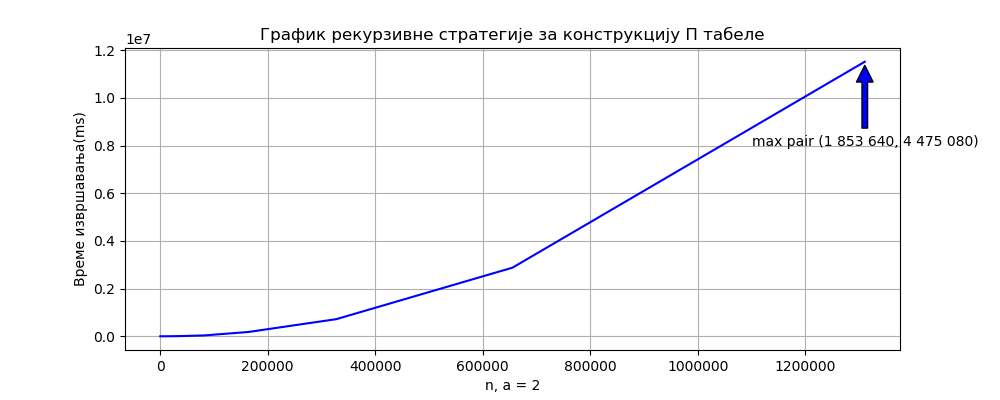
\includegraphics[width=\textwidth]{recursive.png}
	\end{center}
\end{figure}

\subsection{Алгебарска стратегија}

За рзлику од рекурзиивне стратегије која користи имплицитну рекурзију, алгебарска стратегија користи експлицитну рекурзију, рачунајући $ alpha $ и $ beta $. Чиме је укупна временска сложеност конструкције П табеле $ O(n) $.\\

\lstinputlisting[language=C++, linerange={10-24}, caption=Алгебарска стратегија рачунање П табеле]{./src/algebraic.cpp}

\leavevmode\\
Графички приказ зависности $ n $ и времена у милисекундама дат је на \ref{fig:algebraic}, за $ а = 2 $.

\begin{figure}[H]
	\caption{График алгебарске стратегије за конструкцију П табеле}
	\label{fig:algebraic}
	\begin{center}
		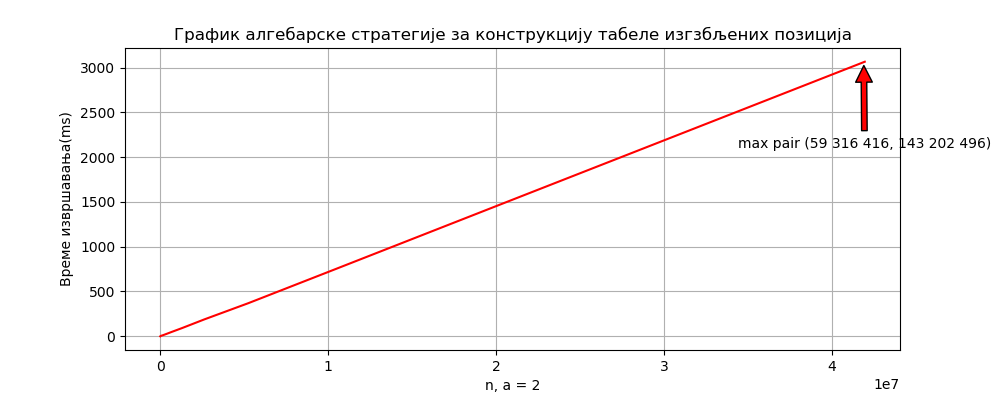
\includegraphics[width=\textwidth]{algebraic.png}
	\end{center}
\end{figure}

\subsection{Аритметичка стратегија}

За раучунање П табеле аритметичком стратегијом прво је потребно конструисати једноставан коначан верижни разломак, што захтева $ O(n) $ времена. 

Потом дефинишемо низове $ p $ и $ q $, њихова димензија је највише $ log(n) $, стога је врeме потребно да дефинишемо ове низове $ O(log(n)) $.

Преостаје још само да $ n $ бројева представимо у $ p $ и $ q $ систему, за њихово представљање у свакој итерацији имамо бинарну претрагу низова $ p $ и $ q $ којом се одређује са колико цифара треба представити број $ i $, што је у најгорем случају једнако величини низова $ p $ и $ q $, тачније $ log(n) $. Тако да је сложеност бинарне претраге $ O(log(log(n))) $. Репрезентација броја $ k $ у $ p $ или $ q $ систему се добија тако што рачунамо количник и остатак дељења броја $ k $ са одгварајућом вредности низа $ p $ или $ q $. Уколико имамо остатак потребно је и њега представити у $ p $ или $ q $ систему, његова $ p $ или $ q $ репрезентација је позната тако да је потребно само да је прекопирамо на крај текуће $ p $ или $ q $ репрезентације броја $ k $, не мењајући притом унапред дефинисан број цифара. Сложеност операције копирања једнака је броју елемената који се копира, што је у најгорем случају $ log(k) - 1 $ цифара. Како имамо $ n $ итерација укупна сложеност представљања првих $ n $ бројева у $ p $ и $ q $ систему захтева $ O(n(log(log(n)) + log(n) - 1)) $ времена.

Чиме је укупна временска сложеност конструкције П табеле $ O(nlog(n)) $

\lstinputlisting[language=C++, linerange={14-94}, caption=Аритметичка стратегија рачунање П табеле]{./src/arithmetic.cpp}

\leavevmode\\
Графички приказ зависности $ n $ и времена у милисекундама дат је на \ref{fig:arithmetic}, за $ а = 2 $.

\begin{figure}[H]
	\caption{График аритметичке стратегије за конструкцију П табеле}
	\label{fig:arithmetic}
	\begin{center}
		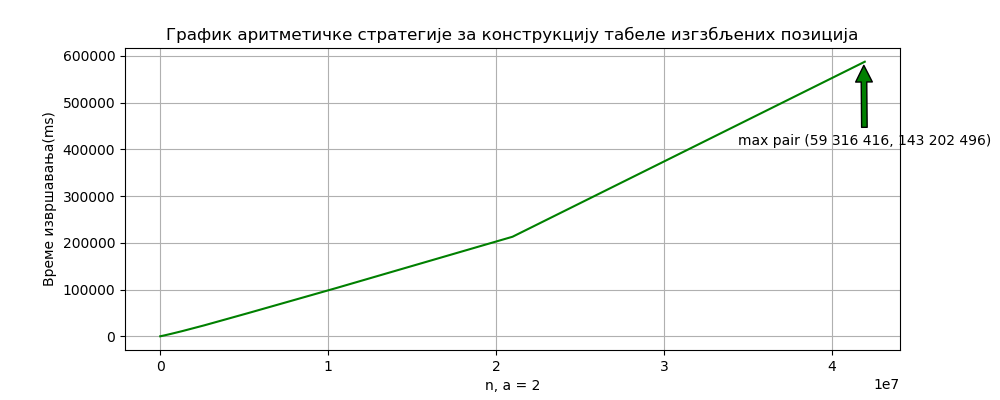
\includegraphics[width=\textwidth]{arithmetic.png}
	\end{center}
\end{figure}

\subsection{Сумиран приказ времена извршавања свих стратегија}

Из претходне анализе се може закључити да је алгебарска стратегија најефикаснија, што се може видети и на обједињеним графицима \ref{fig:all} и  \ref{fig:algebraicVSarithmetic}.

\begin{figure}[H]
	\caption{Сумиран приказ извршавања свих стратегија за конструкцију П табеле}
	\label{fig:all}
	\begin{center}
		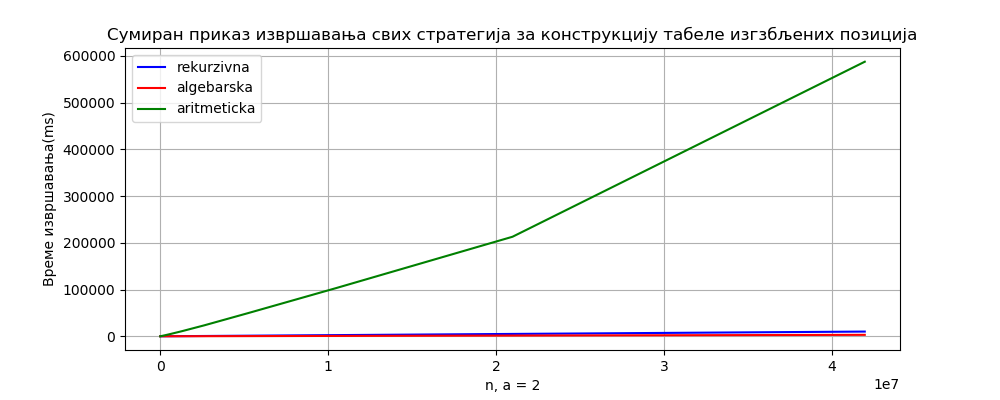
\includegraphics[width=\textwidth]{all.png}
	\end{center}
\end{figure}

\begin{figure}[H]
	\caption{Сумиран приказ извршавања алгебарске и аритметичке стратегије за конструкцију П табеле}
	\label{fig:algebraicVSarithmetic}
	\begin{center}
		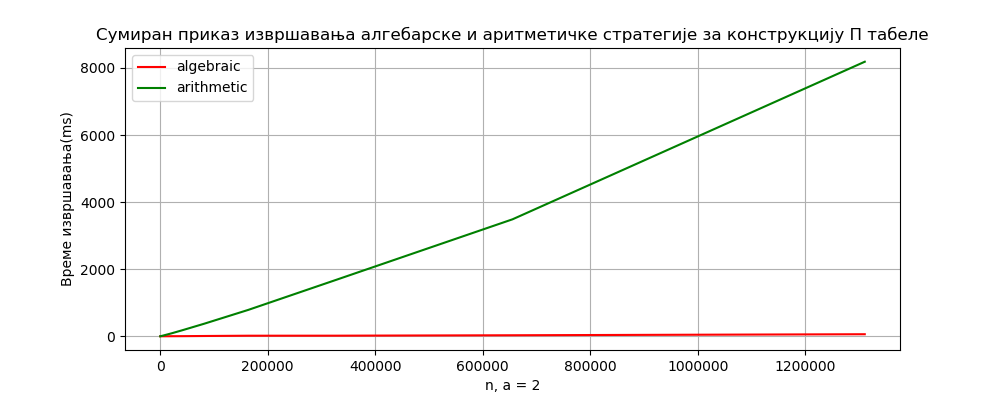
\includegraphics[width=\textwidth]{algebraicVSarithmetic.png}
	\end{center}
\end{figure}

\subsection{Препознавање природе тренутне позиције}

Када имамо израчунате П-позиције, можемо да анализирамо природу тренутне позиције и да одредимо следећу позицију игре.

\lstinputlisting[language=C++, linerange={30-58}, caption= Достизање П позиције рекурзивном и алгебарском стратегијом]{./src/recursive_and_algebraic.cpp}

\appendix
\section{Додатак резултатима}

\csvautolongtable[
table head=\caption{Времена извршавања конструкције П табеле}\label{tab:calculate_time_n}\\\hline
\csvlinetotablerow\\\hline
\endfirsthead\hline
\csvlinetotablerow\\\hline
\endhead\hline
\endfoot,
respect all
]{./src/statistics/csv/calculate_time_n.csv}

\csvautolongtable[
table head=\caption{Парови жетона П табеле}\label{tab:calculate_piles}\\\hline
\csvlinetotablerow\\\hline
\endfirsthead\hline
\csvlinetotablerow\\\hline
\endhead\hline
\endfoot,
respect all
]{./src/statistics/csv/calculate_piles.csv}

\addcontentsline{toc}{section}{Литература}
\appendix
\bibliography{literatura} 
\bibliographystyle{plain}


\end{document}
